\documentclass[11pt,letterpaper]{article}
\usepackage[top=2.0cm, bottom=3cm, left=2.0cm, right=2.0cm]{geometry}
\usepackage[utf8]{inputenc}
\usepackage[T1]{fontenc}
\usepackage[spanish]{varioref}
\usepackage[activeacute, spanish, es-tabla]{babel}
\usepackage{fancyhdr}
\usepackage{multicol}
\usepackage{float}
\usepackage{textcomp}
\usepackage{ae,aecompl}
\usepackage{amssymb,amsmath}
\usepackage[pdftex]{graphicx}
\pagestyle{fancy} 
\pagenumbering{arabic} 
\renewcommand{\headrulewidth}{0pt} 
\setlength{\headsep}{20pt} 
\setlength{\headheight}{65pt} 
\setlength{\textheight}{600pt} 
\setlength{\columnsep}{15pt} 
\newcommand{\universidad}{\small{Universidad Técnica Federico Santa María}}
\newcommand{\campus}{\small{Campus Santiago San Joaquín}}
\newcommand{\semestre}{\small{Segundo Semestre 2016}}

% Definiciones de Título e Integrantes de Experiencia
\newcommand{\titulo}{Tarea 2 - TALF}
\newcommand{\integrantes}{\begin{tabular}{c}
Jorge Contreras 201573547-6 \\
Juan Pablo Jorquera  201573533-6 \\
\end{tabular}}

\renewcommand{\maketitle}
{
\thispagestyle{fancy}
\begin{center}
\begin{Large}
\textbf{\titulo}\\
\end{Large}
\vspace{0.5cm}
\integrantes
\end{center}
\vspace{0.3cm}
}


%ENCABEZADO

\fancyhead[R]{\begin{minipage}[b]{0.405\textwidth}
\begin{center}
\universidad \\ 
\campus \\ 
\lab \\ 
\semestre
\end{center}
\end{minipage}}
\fancyhead[L]{\vspace{15pt}
\includegraphics[height=1.6cm]{Escudo.png}}
%%%%%%%%%%%%%%%%%%%%%%%%%%%%%%%%%%%%%%%%%%%%%%%%
%                                              %
% AQUI TERMINAN LAS DEFINICIONES DE ENCABEZADO %
% Y EMPIEZA EL CUERPO DEL DOCUMENTO            %
%                                              %
%%%%%%%%%%%%%%%%%%%%%%%%%%%%%%%%%%%%%%%%%%%%%%%%

\begin{document}
\maketitle

\section{Pregunta 1}
Primero realizamos el AFD de la tabla para poder trabajar sobre él.

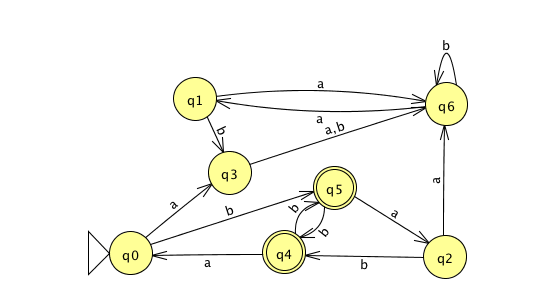
\includegraphics[height=5cm]{tarea_1.png}
\subsection{Parte (a)}
Primero hacemos la tabla correspondiente al autómata.

\begin{table}[h]
\centering
\label{tabla_min}
\begin{tabular}{lllllll}
q1 & X  &    &    &    &    &    \\
q2 & O  & X  &    &    &    &    \\
q3 & X  & O  & X  &    &    &    \\
q4 & X  & X  & X  & X  &    &    \\
q5 & X  & X  & X  & X  & O  &    \\
q6 & X  & O  & X  & O  & X  & X  \\
   & q0 & q1 & q2 & q3 & q4 & q5
\end{tabular}
\caption{Tabla de equivalencias}
\end{table}

Luego continuamos eliminando los que son equivalentes:
\newpage
\begin{itemize}
\item{Eliminar q2:}

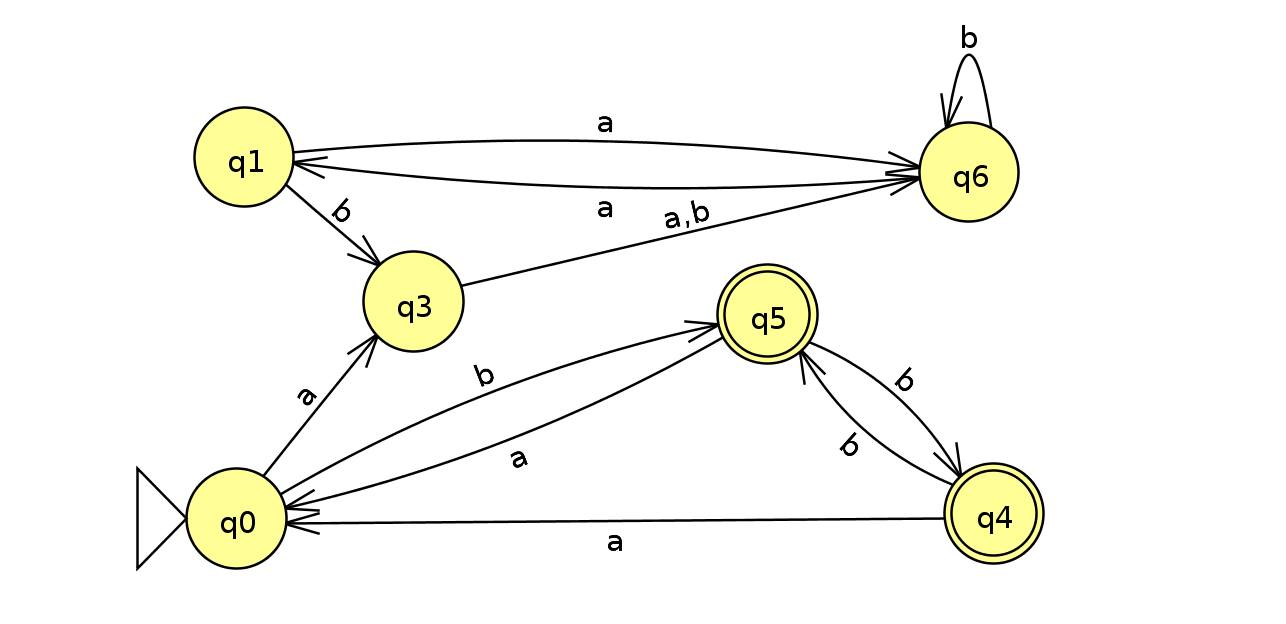
\includegraphics[height=5cm]{tarea_1-a.png}

\item{Eliminar q5:}

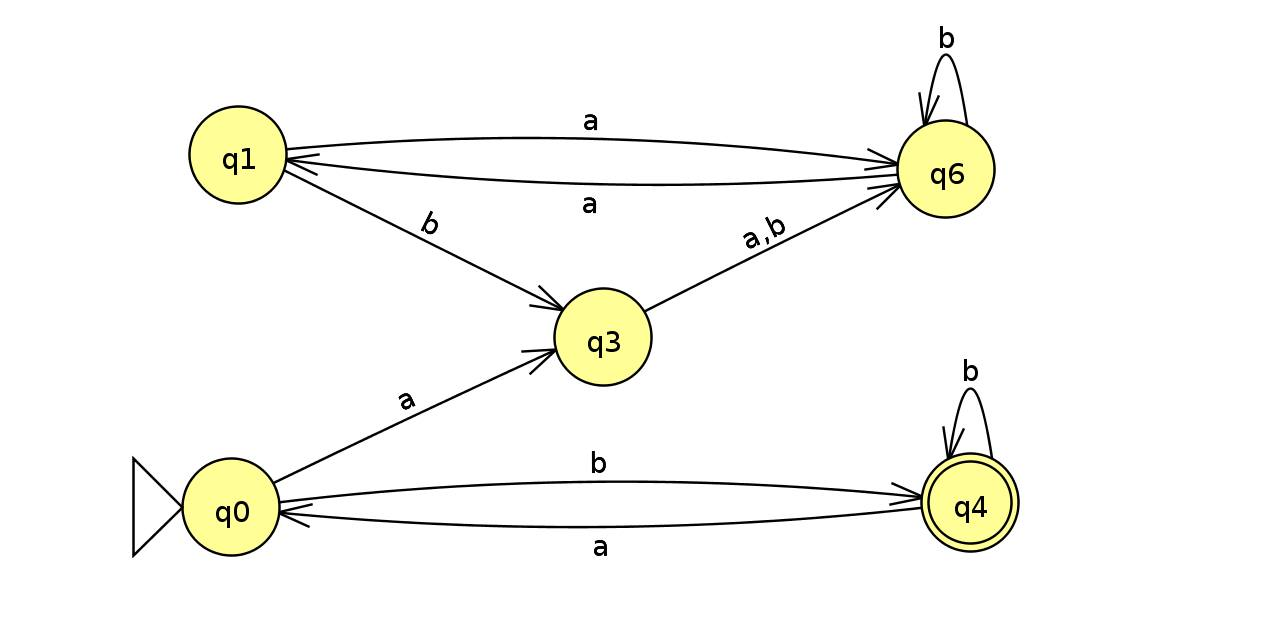
\includegraphics[height=5cm]{tarea_1-a-2.png}

\item{Eliminar q3:}

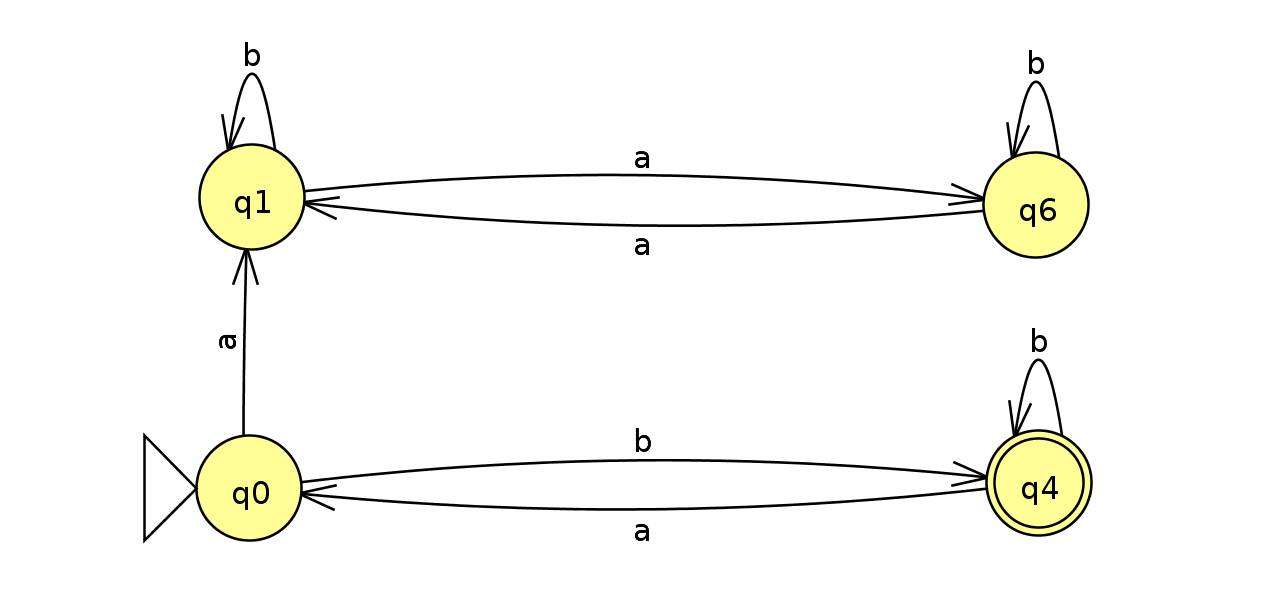
\includegraphics[height=5cm]{tarea_1-a-3.png}
\newpage
\item{Eliminar q6:}

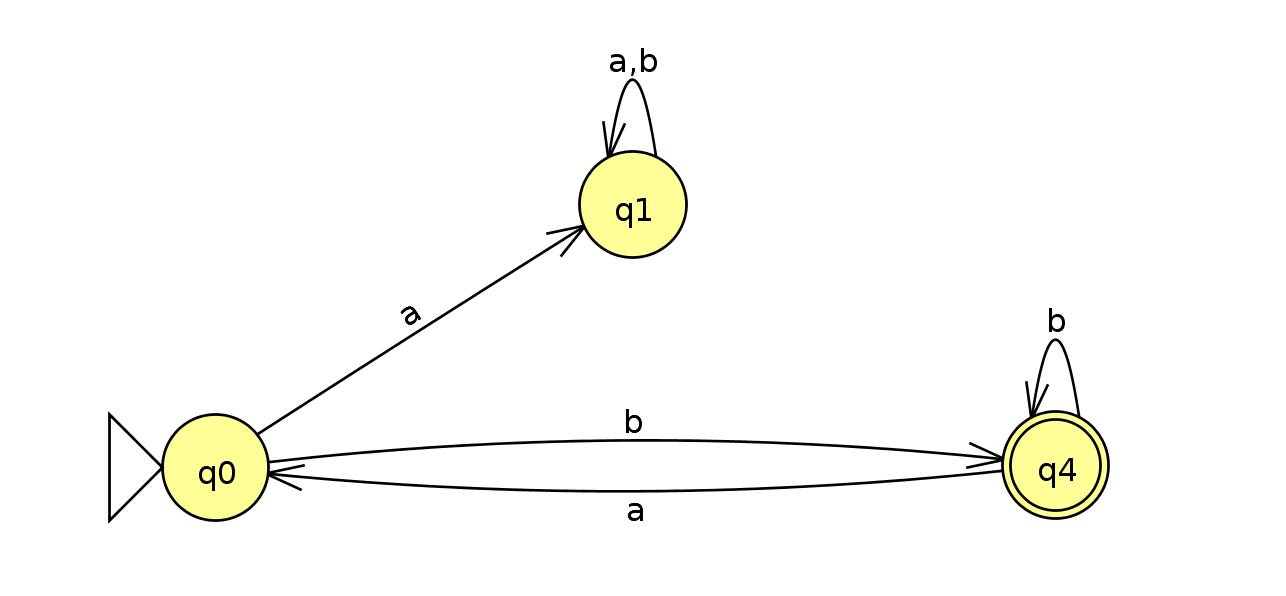
\includegraphics[height=5cm]{tarea_1-a-4.png}
\end{itemize}


\subsection{Parte (b)}
\begin{itemize}
	\item{Tomando q0 y q1: la palabra ``b'' distingue a ambos, ya que quedan en distinto estado de aceptación.}
	\item{Tomando q0 y q4: simplemente ``a'' los distingue.}
	\item{Tomando q1 y q4: ``ab'' los distingue.}
\end{itemize}

\subsection{Parte (c)}
\begin{itemize}
\item{Primero normalizamos para tener un nodo de entrada y de salida claros.}
\begin{center}
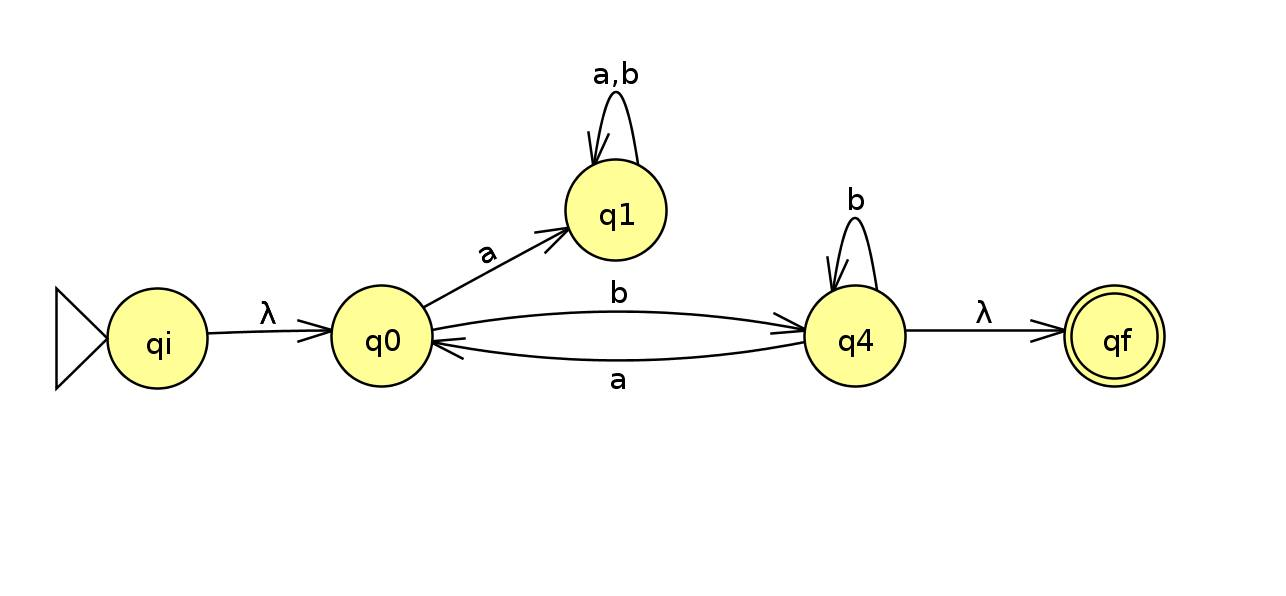
\includegraphics[height=4.3cm]{tarea_1-c.png}
\end{center}
\item{Luego eliminamos el nodo ``basura'' que se encuentra.}
\begin{center}
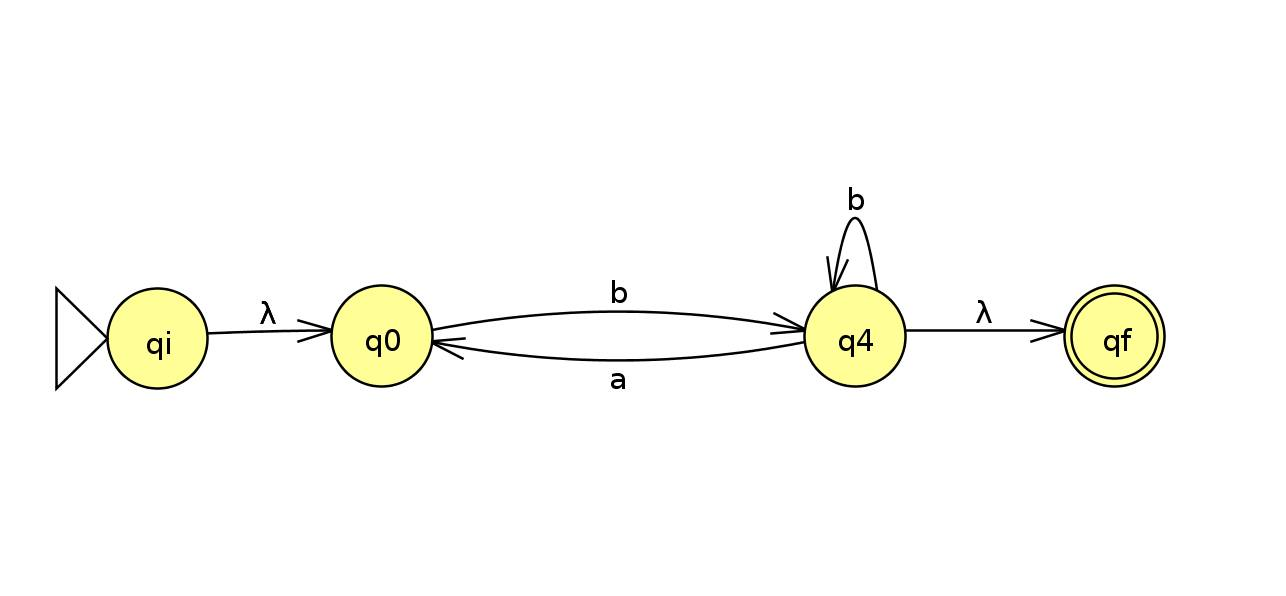
\includegraphics[height=4.3cm]{tarea_1-c2.png}
\end{center}
\item{Eliminamos q4.}
\begin{center}
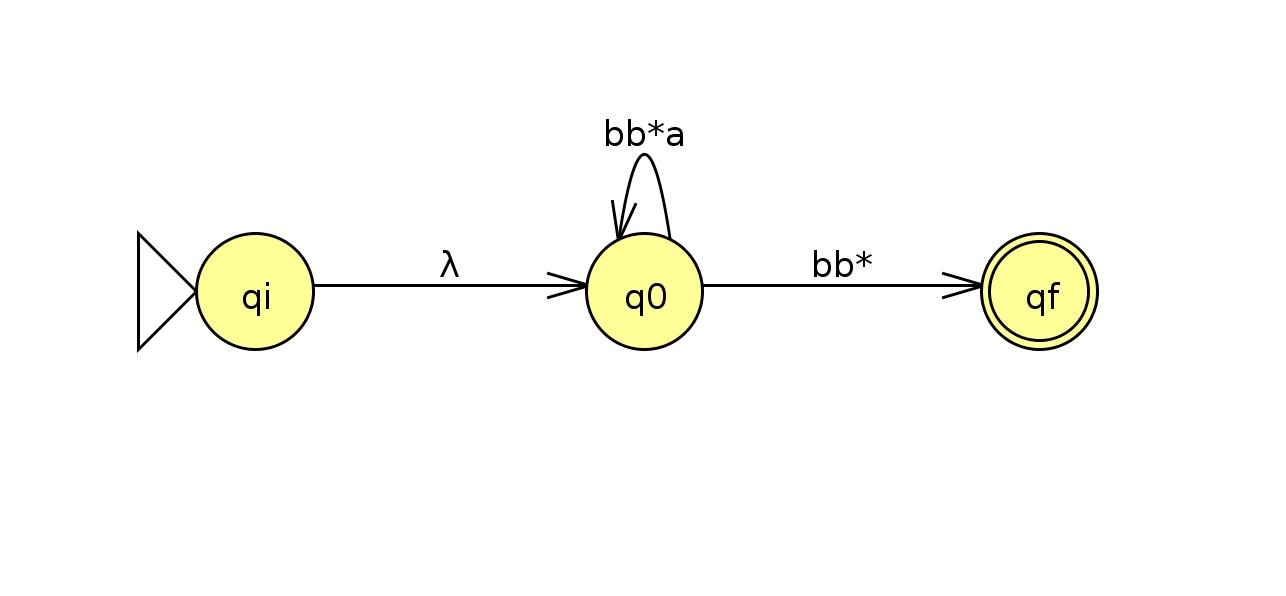
\includegraphics[height=4.3cm]{tarea_1-c3.png}
\end{center}
\item{Finalmente eliminamos q0.}
\begin{center}
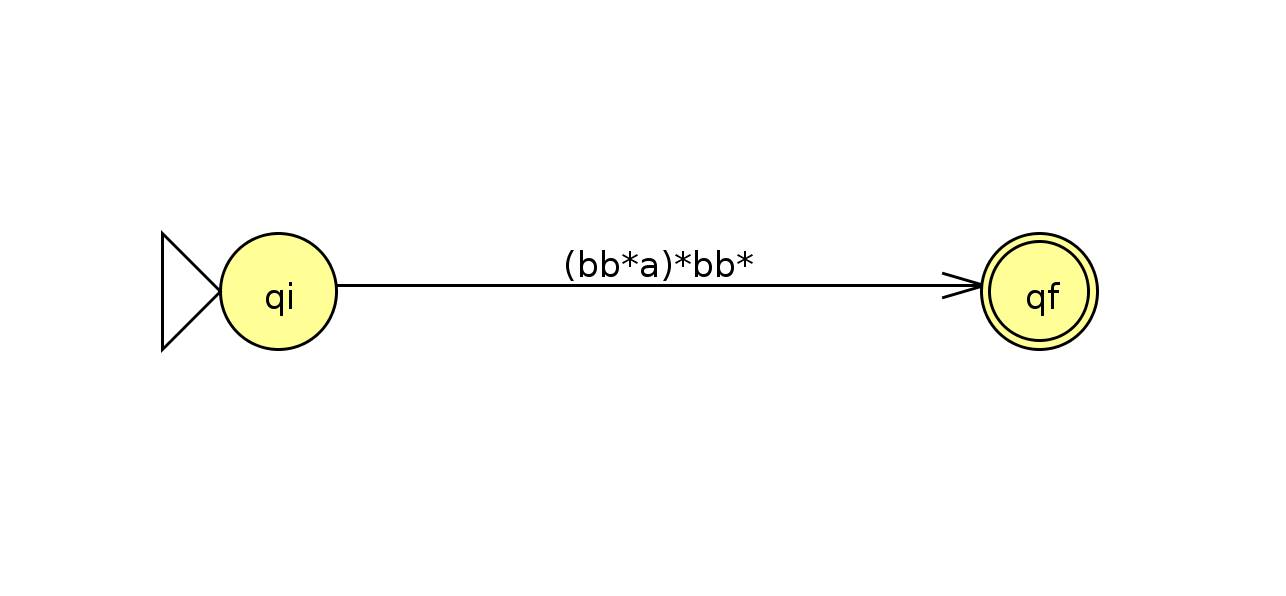
\includegraphics[height=4.3cm]{tarea1-c4.png}
\end{center}
\end{itemize}

\subsection{Parte (d)}
Corresponde al lenguaje que comienza con una o más ``b'' y, si lo sigue una ``a'', se repite el proceso con ``b'' nuevamente.

\section{Pregunta 2}
\subsection{Parte (a)}
\begin{itemize}
\item{Pertenece: baabba}
\item{No Pertenece: bababa}
\end{itemize}
\subsection{Parte (b)}
Al estar w definido en el alfabeto $\Sigma$, podemos decir que |w| = a con a > 0, por lo que al concatenar, los largos |ww| = 2a ; |www| = 3a y como a > 0, entonces |ww| siempre será distinto a |www|, por lo que dicho lenguaje es vacío.
\subsection{Parte (c)}
Como u y v pertenecen a $\Sigma ^*$ podemos tomar el caso particular de u = v = $\epsilon$, en dicho caso la regla para w sería equivalente a: w = w; lo que sabemos se cumple siempre, por lo que este lenguaje es completo.

\section{Pregunta 3}
\subsection{Parte (a)}
b*(ab*ab*ab*)*
\subsection{Parte (b)}
(b+ab+aab)*aaa(ba+baa+b)*
\subsection{Parte (c)}
(b+ab+aab)*(ba+baa+b)*

\section{Pregunta 4}
\subsection{Parte (a)}
\subsection{Parte (b)}
\subsection{Parte (c)}

\section{Pregunta 5}
\subsection{Parte (a)}
\renewcommand{\thefootnote}{\fnsymbol{footnote}}
\subsection{Parte (b) \protect\footnote{Los nombres de los nodos fueron puestos como etiquetas para evitar problemas de visibilidad. asdasd}}


\newpage
\subsection{Parte (c)}

El estado inicial (q0q1q2q3) del AFD es de aceptación, lo que significa que acepta la palabra vacía. Como sabemos que la expresión regular acepta “ab”, “aab” o “aba” tantas veces como se requiera, para llegar al segundo estado (q4q5q6) se requiere de una “a”, y como “a” no pertenece a la expresión regular, este no es un estado de aceptación. Luego, Si se ingresa una “b” se llega a una palabra aceptada por la expresión, por lo cual es estado de aceptación (q0q1q2q3q7q9), si en su defecto se elige “a”, se llega a un estado de no aceptación (q8), ya que “aa” no pertenece a la expresión. \\

Siguiendo ahora desde el estado q0q1q2q3q7q9 con “a” se llega al siguiente estado (q0q1q2q3q4q5q6q11) donde sí hay aceptación dado que se formaría “aba”, la cual pertenece a la expresión, desde este estado si se elige “b” se vuelve al nodo q0q1q2q3q4q7q9, generando un ciclo, porque se repite la expresión “ab” dos veces, siendo esto aceptado. Si por el contrario se opta por “a” se llega al estado q4q5q6q8 que no es de aceptación dado que “abba” no pertenece a la expresión regular. \\

Desde q8 se puede llegar a q0q1q2q3q10 con “b”, formando la palabra “aab” que pertenece a la expresión, por esto es que es estado de aceptación. \\

El estado q4q5q6q8 no es de aceptación, tal como se mencionó anteriormente, y eligiendo “a” se va al estado q8 que es el estado de basura,  eligiendo en cambio “b” se llega al estado q0q1q2q3q7q9q10 que es de aceptación ya que al llegar a él se forma la palabra “abaab” que es la concatenación de “ab” y “aab”, lo cual es aceptado. Desde este se llega nuevamente al estado q0q1q2q3q4q5q6q11 mediante “a”, y es nuevamente estado de aceptación dado que la palabra al llegar sería “abaaba” que es “aba” dos veces, lo cual es aceptado. \\

Estando todos los estado ya descritos, las demás posibles  interacciones y ciclos se deben sólo a que la expresión regular que finaliza con *, significando que se puede hacer el mismo proceso infinitas veces.

\end{document}
